\subsubsection{Klassebeskrivelser}

\bigskip
\bigskip
\textbf{Communications} namespacet indeholder klasser der gør det muligt at skabe forbindelse til \gls{CS} .\\

\textbf{Client}
Denne benytter singleton-klassen \textit{LSC}\footnote{LSC findes på side \pageref{LSC_Beskrivelse}.} til at oprette forbindelse til \gls{CS} og sende data igennem denne. Det er denne klasse som bruges i bl.a. ModelHandleren{\footnote{ModelHandler findes på side \pageref{Modelhandler_Beskrivelse}.}} til at sende data.
\begin{center}
\begin{figure}[!h]
    \centering
    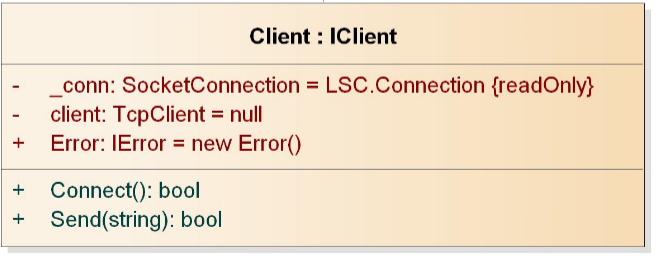
\includegraphics[width=0.55\textwidth]{Systemdesign/backend/klassebeskrivelser/Images/Client.png}
    \caption{Client}
    \label{fig:Client}
\end{figure}
\end{center}
\label{Client_Beskrivelse}
 \bigskip 


\textbf{LSC}
\label{LSC_Beskrivelse}\\
LSC er en wrapper-klasse som indkapsulerer en socketforbindelse fra \gls{SL} som en singleton. Singleton benyttes således at uanset hvilken instans af  client i programmet der bruges, vil den samme forbindelse blive brugt. 
\begin{center}
\begin{figure}[!h]
    \centering
    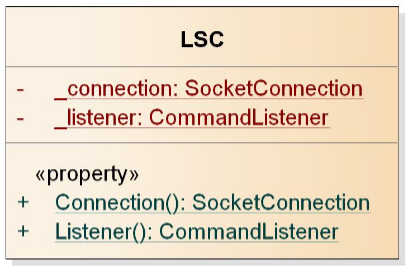
\includegraphics[width=0.30\textwidth]{Systemdesign/backend/klassebeskrivelser/Images/LSC.png}
    \caption{LSC }
    \label{fig:LSC}
\end{figure}
\end{center}
\label{LSC_Beskrivelse}
 \bigskip 
